\FloatBarrier
\subsection{Question 1}
\autoref{code:pp11} outlines the steps required to plot the zero and pole locations for both continuous and discrete systems. The resulting plots are shown in \autoref{fig:pp11} for the continuous system and \autoref{fig:pp12} for the discrete system.

\begin{code}
	\begin{matlabcode}{firstnumber = 8}
fprintf('Roots of continues transfer function:\n');
continuesRoots = roots(G_Original.den{1});
display(continuesRoots);
figure;
pzplot(G_Original);
ee = findobj(gca,'type','line');
for i = 1:length(ee)
	set(ee(i),'markersize',24); 
	set(ee(i), 'linewidth',2) ; 
end
xlim([-2 1]);title('Pole-Zero map of continues system');fontsize( 24 ,"points");

fprintf('Roots of discrete transfer function:\n');
discreteRoots = roots(Gz.den{1});
display(discreteRoots);
figure;
pzplot(Gz);
ee = findobj(gca,'type','line');
for i = 1:length(ee)
	set(ee(i),'markersize',24); 
	set(ee(i), 'linewidth',2) ; 
end
title('Pole-Zero map of discrete system');fontsize( 24 ,"points");
	\end{matlabcode}
	\captionof{listing}{Zeros \& poles}
	\label{code:pp11}
\end{code}

\begin{figure}
	\centering
	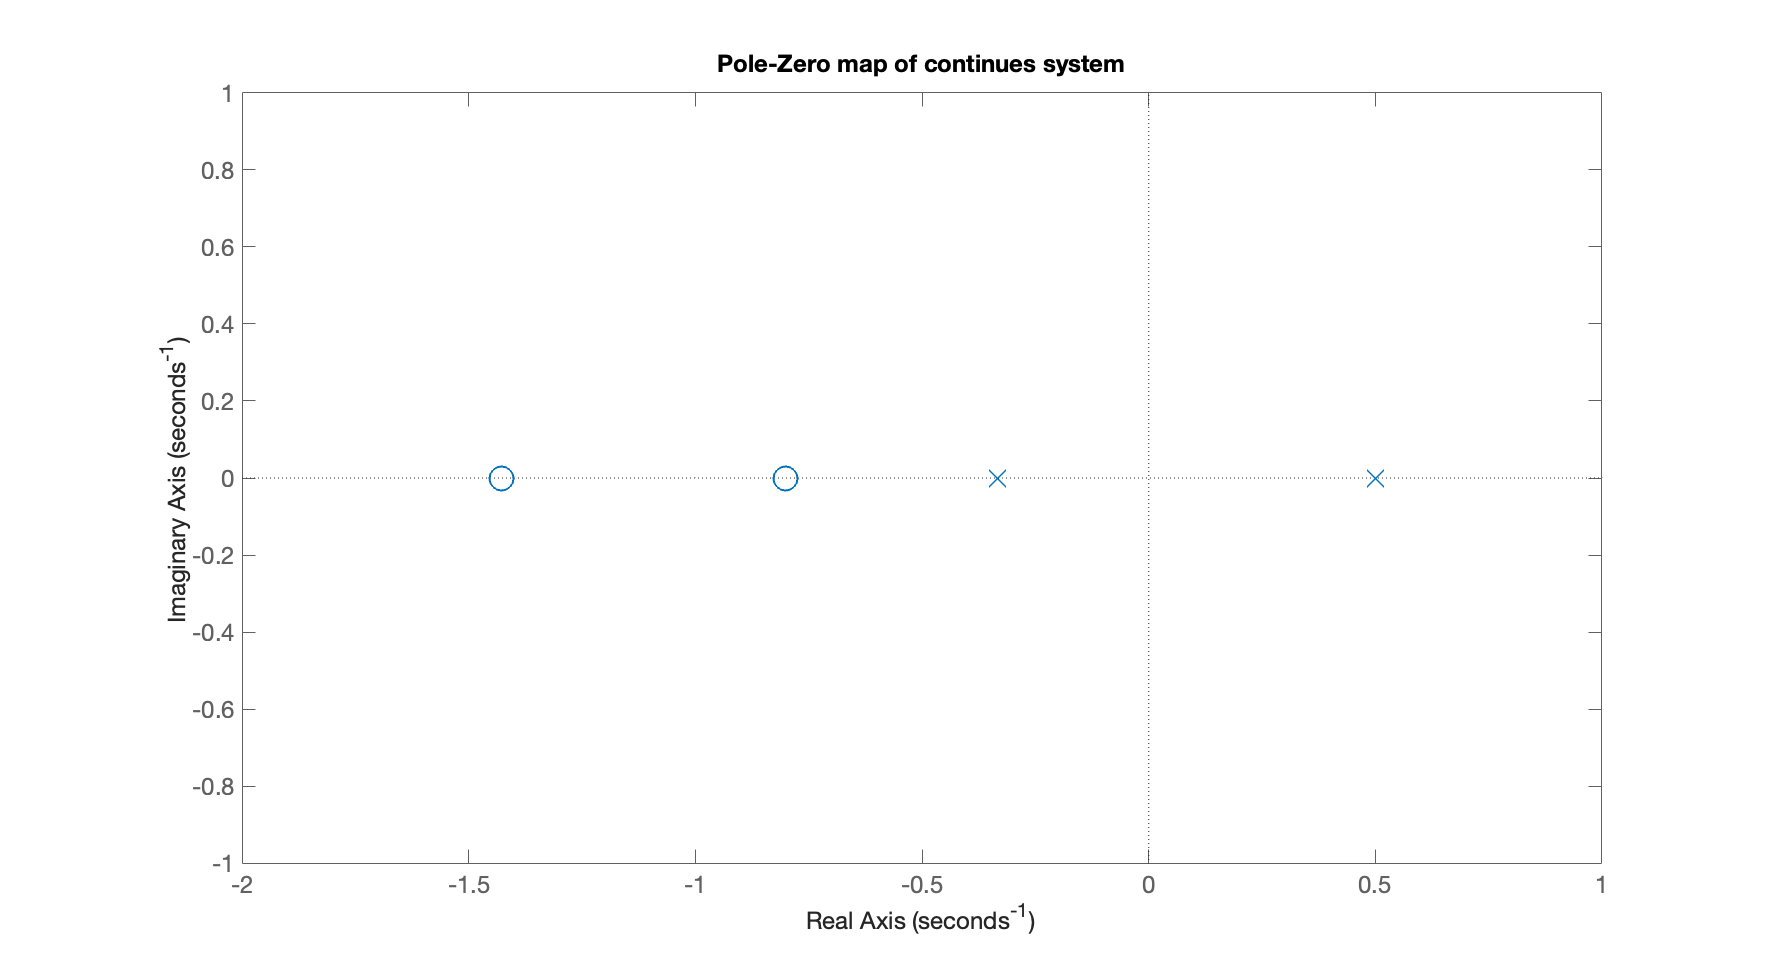
\includegraphics[width=\textwidth]{images/pp11.png}
	\caption{Continues system poles \& zeros}
	\label{fig:pp11}
\end{figure}

\begin{figure}
	\centering
	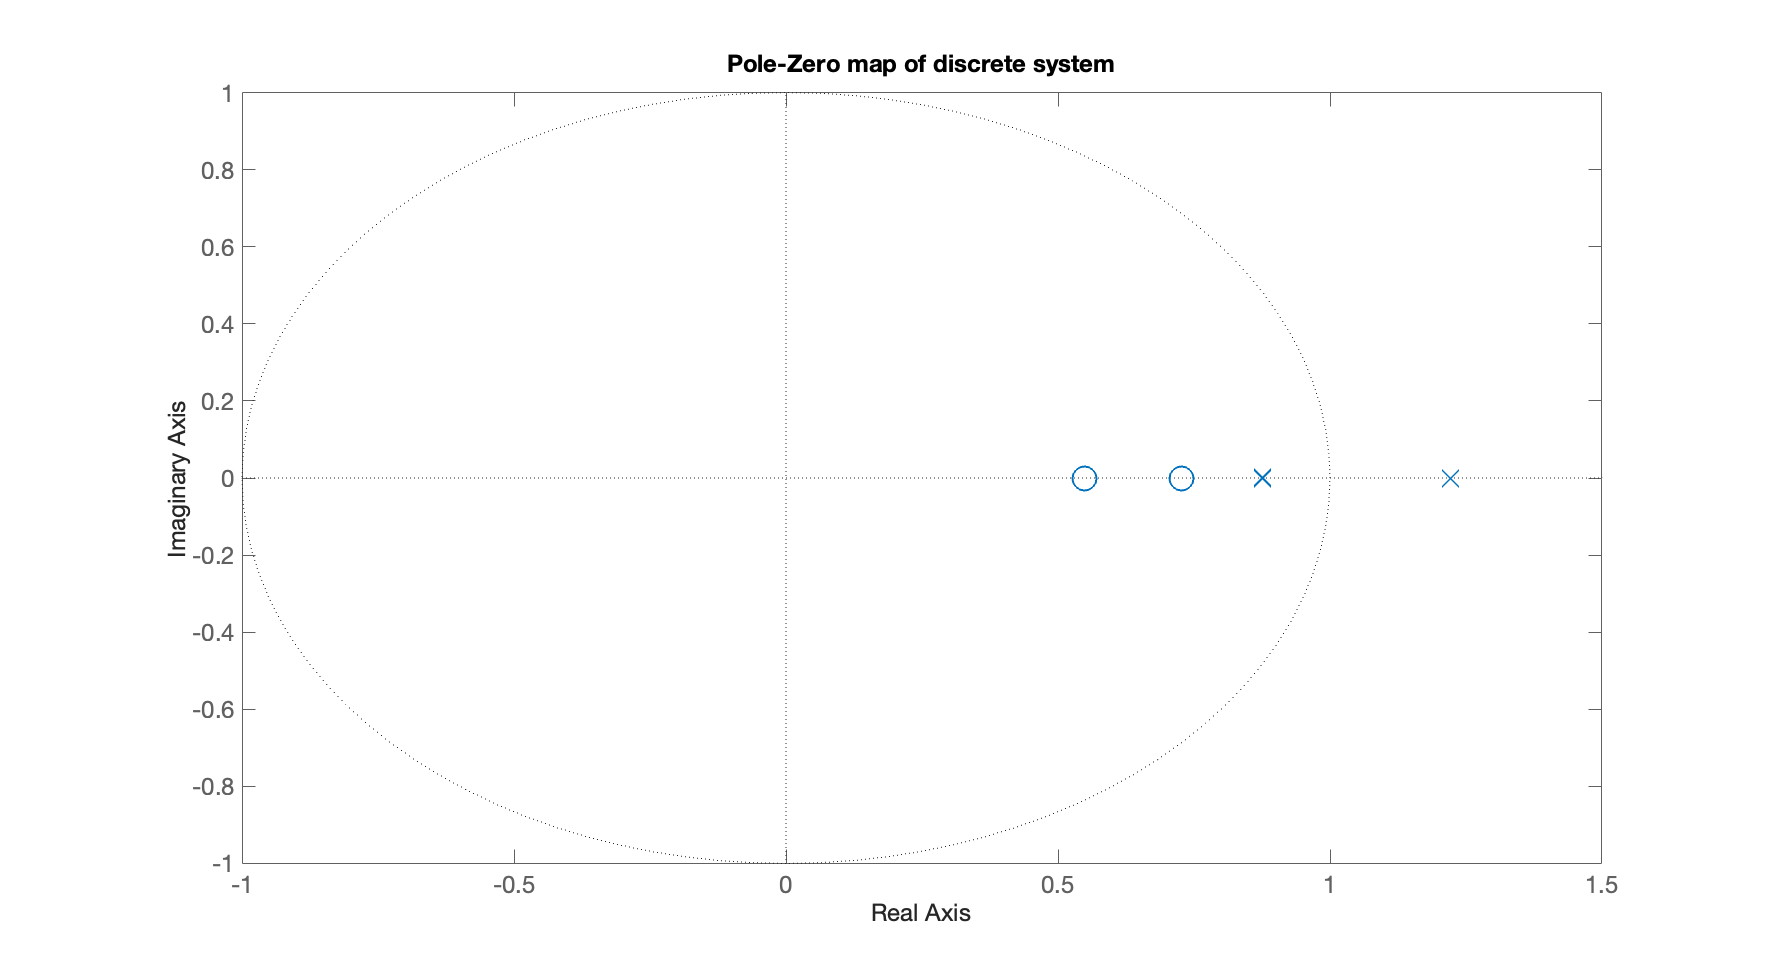
\includegraphics[width=\textwidth]{images/pp12.png}
	\caption{Discrete system poles \& zeros}
	\label{fig:pp12}
\end{figure}

As shown in \autoref{fig:pp12}, the system has a pole located outside the unit circle, indicating that it is unstable. To design our reference model, we will relocate this unstable pole inside the unit circle and determine $B_m$ such that the step response approaches a steady-state value of $1$.

\noindent The code for this section is available at \lstinline|assignment2/part1/PP1_1.m|. 
